Este capítulo tem como objetivo apresentar a metodologia da avaliação de desempenho dos diferentes sistemas de inferência propostos.

%%%%%%%%%%%%%%%%%%%%%%%%%%%%%%%%%%%%%%%%%%%%%%%%%%%%%%%%%%%%%%%%%%%%%%%%%%%%%%%%
%%%%%%%%%%%%%%%%%%%%%%%%%%%%%%%%%%%%%%%%%%%%%%%%%%%%%%%%%%%%%%%%%%%%%%%%%%%%%%%%
%%%%%%%%%%%%%%%%%%%%%%%%%%%%%%%%%%%%%%%%%%%%%%%%%%%%%%%%%%%%%%%%%%%%%%%%%%%%%%%%

\section{Motivação}%

Avaliações são importantes na busca pelo máximo desempenho de um sistema com os recursos disponíveis. Seus resultados auxiliam tanto nas decisões de escolhas entre diferentes sistemas ou simplesmente entender o funcionamento de um sistema já existente.

Devido à grande diversidade de sistemas, não existe um procedimento padrão comum em que seja possível analisar eficientemente um sistema qualquer. Por este motivo é necessário conhecer o sistema a ser avaliado e escolher as métricas, carga de trabalho e técnicas de avaliação apropriadas. \cite{jain1991art}

Em uma simulação, o ONS pode realizar um número significativo de chamadas para obter resultados inferidos de modelos de redes neurais profundas. Um dos modelos de interesse se trata da classificação da qualidade dos algoritmos de alocação de recursos em EONs, tendo como entrada a topologia da rede simulada no ONS.

O objetivo desta avaliação de desempenho é escolher um conjunto de fatores que minimizem principalmente o tempo total percorrido durante o processo de inferência, aqui mencionado como tempo de inferência. Além disso, os resultados de cada inferência serão comparados com os valores esperados de modo a verificar se há perda de acurácia em certas combinações de fatores.

%%%%%%%%%%%%%%%%%%%%%%%%%%%%%%%%%%%%%%%%%%%%%%%%%%%%%%%%%%%%%%%%%%%%%%%%%%%%%%%%
%%%%%%%%%%%%%%%%%%%%%%%%%%%%%%%%%%%%%%%%%%%%%%%%%%%%%%%%%%%%%%%%%%%%%%%%%%%%%%%%
%%%%%%%%%%%%%%%%%%%%%%%%%%%%%%%%%%%%%%%%%%%%%%%%%%%%%%%%%%%%%%%%%%%%%%%%%%%%%%%%

\section{Metodologia}%
\label{analysis-motivation}

De acordo com Raj Jain \cite{jain1991art}, há três métodos de avaliação de desempenho: modelagem analítica, simulação e medição.

O sistema a ser avaliado, devido à presença de modelos de redes neurais profundas, é complexo o suficiente para tornar a modelagem analítica inviável. Além disso, uma instância de simulação do ONS pode levar horas para ser finalizada, inviabilizando também a escolha do método de medição. Sendo possível simular apenas a execução do ONS responsável por inferir a partir de modelos de inteligência artificial, a avaliação de desempenho será então realizada através de simulações.

A simulação será executada em um programa Java, representando a seção do ONS responsável por receber a entrada apropriada (e.g. topologia da rede simulada) e realizar a inferência. Java é a linguagem escolhida por ser a linguagem em que o ONS é desenvolvido. Este programa será responsável por carregar a carga de trabalho em memória e realizar múltiplas inferências, registrando o resultado e o tempo de execução de cada uma.

Nesta avaliação, serão consideradas duas opções para a realização da inferência:

\begin{itemize}
  \item \textbf{Programa externo escrito em Python}. Como é possível ver na figura \ref{fig:languagesml}, entre desenvolvedores da área, Python é a linguagem mais usada e priorizada para desenvolvimento em inteligência artificial. Os desenvolvedores dos modelos de inteligência artificial do grupo de pesquisa COMNET utilizam primariamente Python, um aspecto importante ao considerar futuras manutenções e implementações de sistemas de inferência.
  \item \textbf{Módulo interno em Java}. Devido ao fato do ONS ser escrito em Java, sistemas de inferência em Python seriam necessariamente externos, necessitando-se então a implementação de comunicação entre os processos. O tempo extra ocupado pela transferência dos dados de saída e entrada do sistema de inferência pode se tornar um gargalo de desempenho. Deste modo executar a inferência no mesmo processo poderia resultar em um ganho significativo de tempo de inferência.
\end{itemize}

\begin{figure}[h]
  \centering
  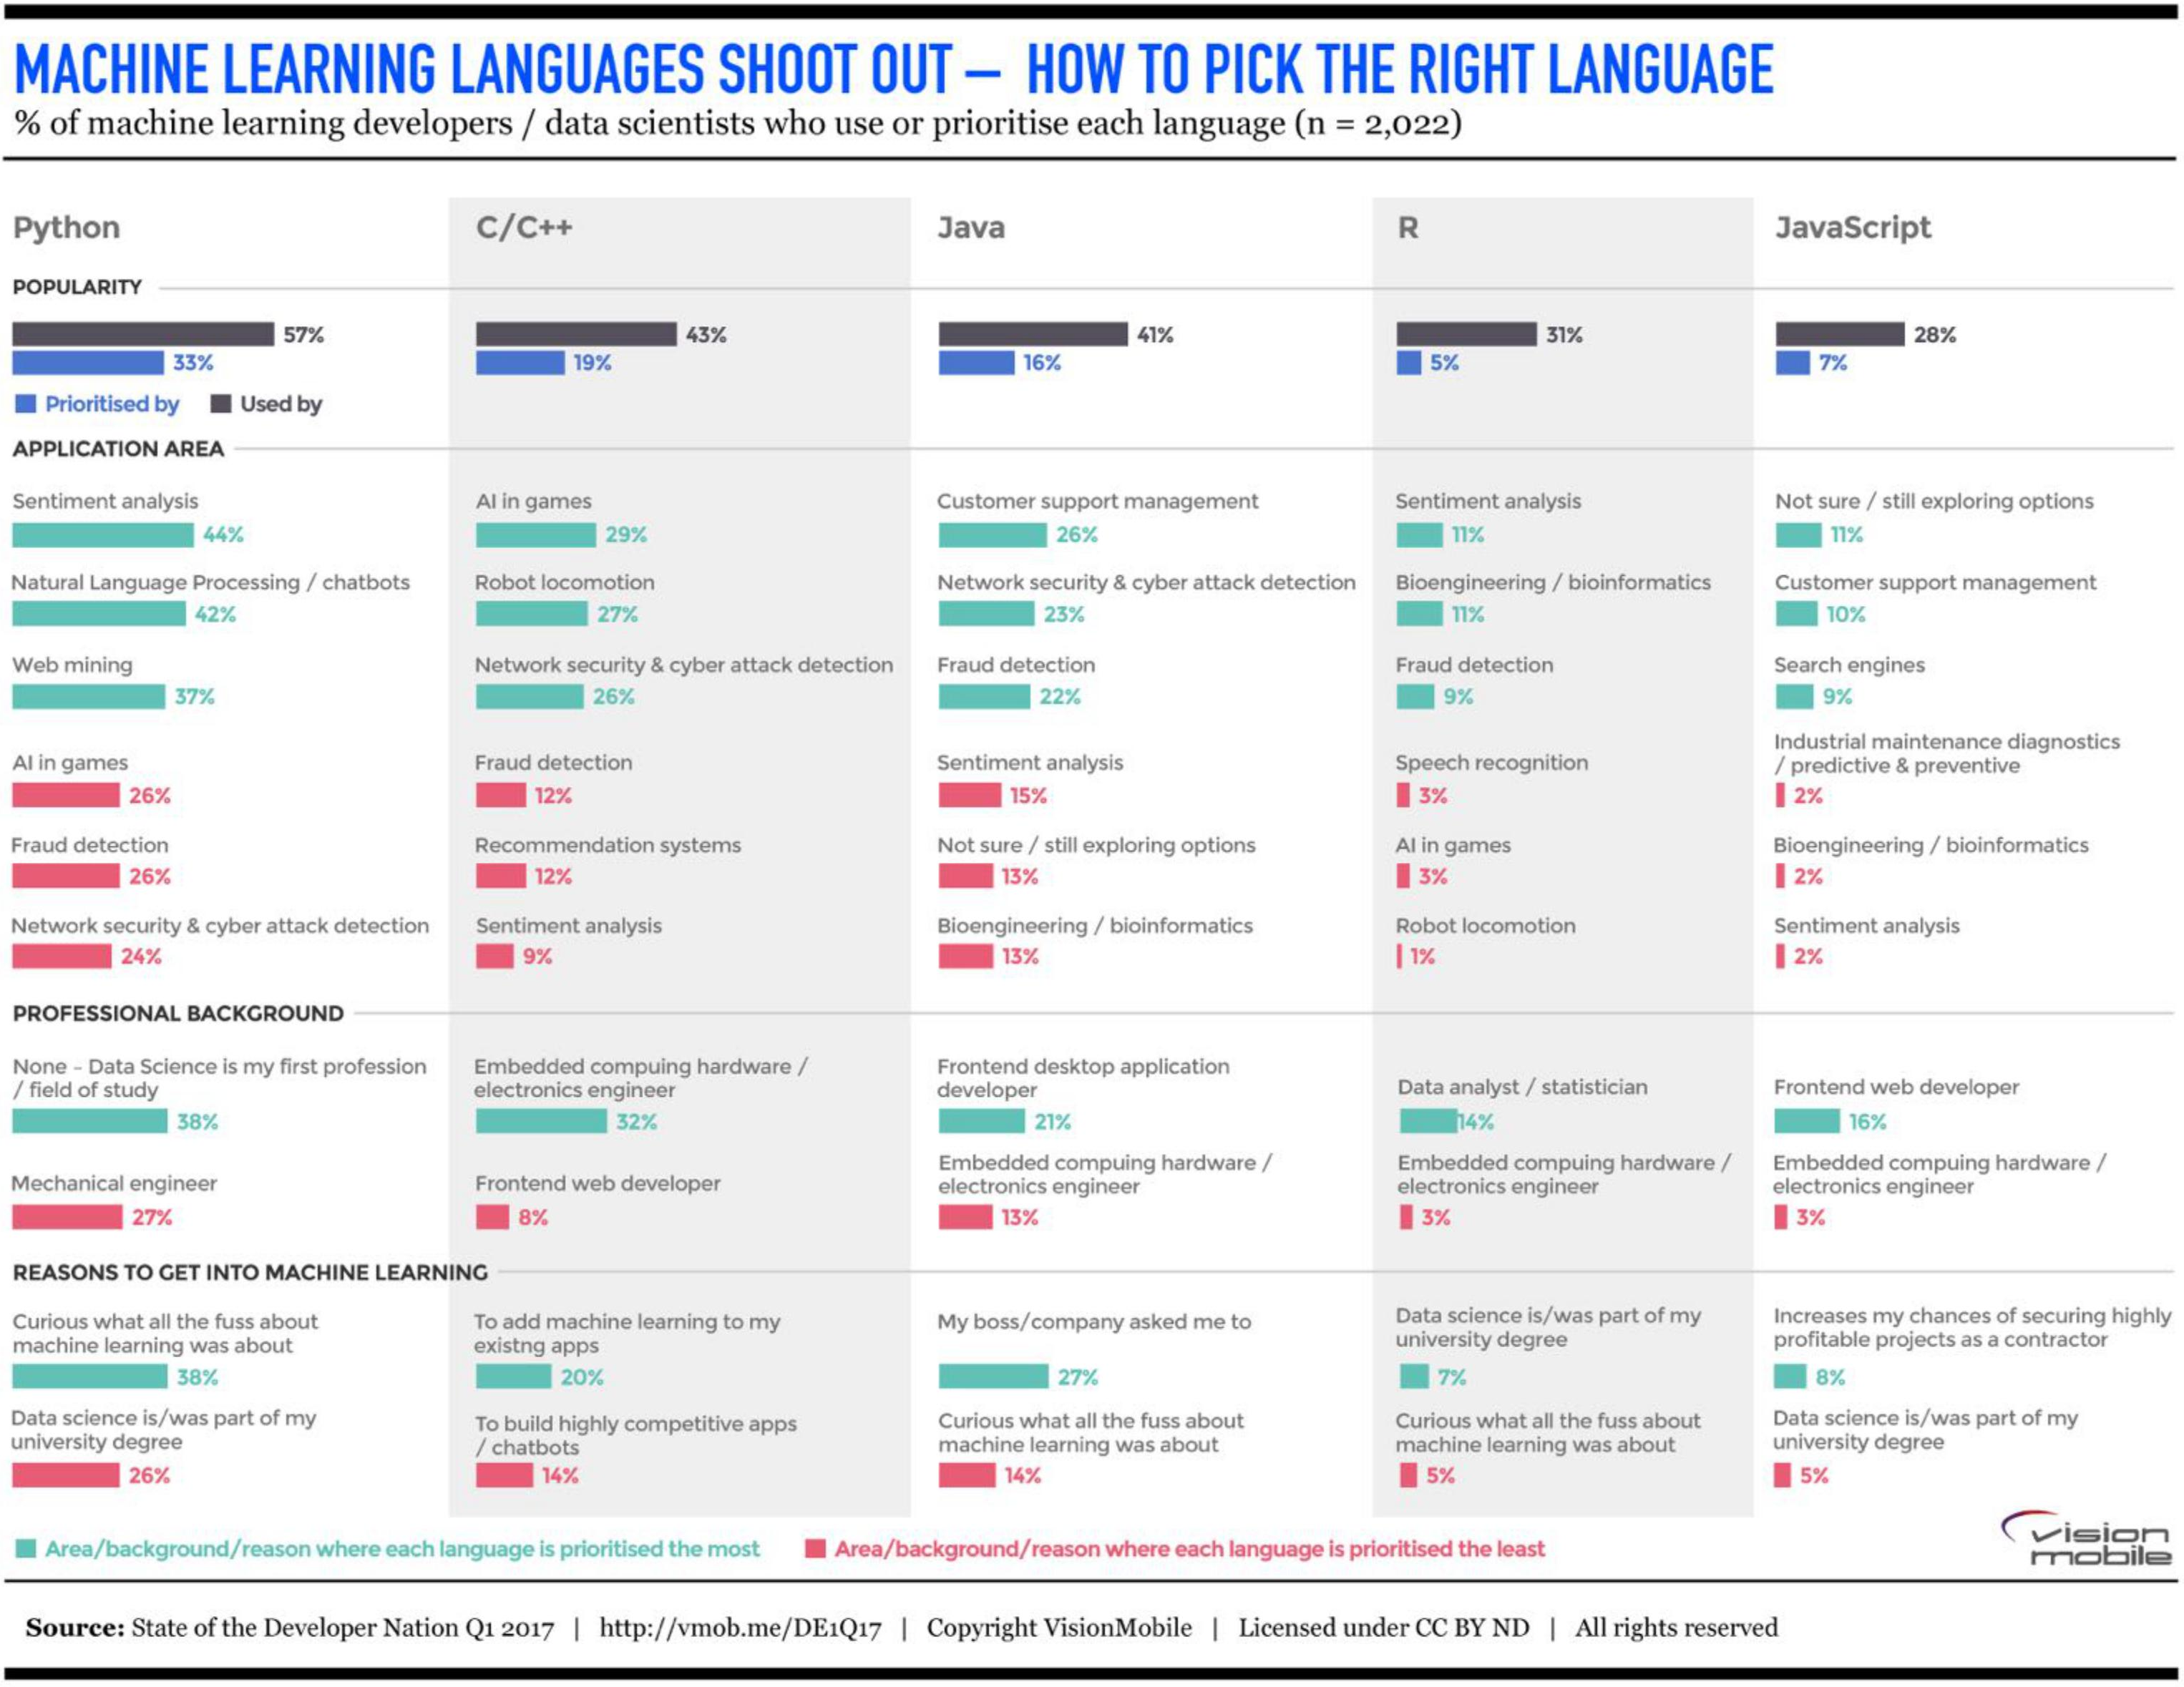
\includegraphics[width=1\textwidth]{img/languages-ml.png}
  \caption{Porcentagem de cientistas de dados e desenvolvedores de inteligência artificial que usam ou priorizam cada linguagem \cite{developer_nation_q1_2017}}
  \label{fig:languagesml}
\end{figure}

Neste estudo, com o objetivo de analisar o impacto de cada um dos fatores descritos na seção \ref{paramsfactors}, será realizado um desenho experimental do tipo fatorial completo, onde é realizada uma simulação para cada combinação diferente dos fatores. O principal benefício deste tipo de desenho experimental é a possibilidade de analisar o impacto individual dos fatores assim como impactos de combinações específicas de um subconjunto dos fatores.

%%%%%%%%%%%%%%%%%%%%%%%%%%%%%%%%%%%%%%%%%%%%%%%%%%%%%%%%%%%%%%%%%%%%%%%%%%%%%%%%
%%%%%%%%%%%%%%%%%%%%%%%%%%%%%%%%%%%%%%%%%%%%%%%%%%%%%%%%%%%%%%%%%%%%%%%%%%%%%%%%
%%%%%%%%%%%%%%%%%%%%%%%%%%%%%%%%%%%%%%%%%%%%%%%%%%%%%%%%%%%%%%%%%%%%%%%%%%%%%%%%

\section{Métricas}

Em uma execução comum de uma simulação do ONS, a inferência de um modelo pode ser requisitada até centenas de milhares de vezes, de acordo com o contexto. Este comportamento torna as seguintes métricas de desempenho importantes:

\begin{itemize}
  \item \textbf{Tempo de inferência} — o tempo total percorrido desde a chamada do serviço de inferência até a obtenção do resultado. Pelo possível alto número de chamadas realizadas por uma execução do ONS, é crucial que cada chamada tome o menor tempo possível para diminuir o tempo de execução total do ONS;
  \item \textbf{Acurácia} — taxa de acerto dos resultados das inferências, comparado com o resultado esperado. O resultado de uma inferência impacta as ações da simulação sendo executada no ONS, tornando importante avaliar se certas combinações de fatores do sistema diminuem a acurácia do serviço de inferência para um valor abaixo do esperado.
\end{itemize}

\section{Parâmetros e Fatores}
\label{paramsfactors}

Em uma análise de desempenho, é importante estar ciente dos parâmetros do sistema que podem afetar o desempenho do serviço \cite{jain1991art}. Os parâmetros são categorizados de duas maneiras: os que serão variados durante a avaliação e os que não serão. Os variados são chamados de \textbf{fatores} e seus valores de \textbf{níveis}.

De acordo com a definição do sistema e as métricas de avaliação, são conhecidos os seguintes parâmetros, com suas definições descritas, com possível impacto nos resultados:

\begin{itemize}
  \item Velocidade da CPU — Intel Core i3-8100;
  \item Velocidade da GPU — GeForce RTX 2060;
  \item Número e tamanho de parâmetros de chamada — definidos na seção \ref{workload};
  \item Linguagem de programação usada para a inferência;
  \item Framework usada para a inferência;
  \item Uso da CPU ou da GPU para a inferência;
  \item Modelo de inteligência artificial usado na inferência — classificação da qualidade dos algoritmos de alocação de recursos em EONs, tendo como entrada a topologia da rede simulada no ONS;
  \item Cargas diversas na máquina onde a simulação é feita.
\end{itemize}

Dentre os parâmetros, os seguintes fatores e seus níveis são escolhidos:

\begin{itemize}
  \item \textbf{Uso da CPU ou da GPU para a inferência}. Modelos de redes neurais profundas, dependendo de suas características e como são utilizados, podem beneficiar-se ou não da disponibilidade de uma GPU;
  \item \textbf{Linguagem de programação usada para a inferência} — Java e Python. Descritas na seção \ref{analysis-motivation}.
  \item \textbf{Framework usada para inferência} — fator relacionado com a linguagem de programação, pois algumas frameworks não estão disponíveis para ambas linguagens. Serão simuladas execuções usando as bibliotecas ONNX \cite{onnx2019} (Java e Python), Tensorflow Lite (Python), Tensorflow (Java) e deeplearning4j \cite{deeplearning4j} (Java).
\end{itemize}

Tendo em vista a utilização de um desenho fatorial completo, ao descartar combinações incompatíveis, observa-se que as combinações destes fatores resultam em 10 simulações diferentes.

\section{Carga de Trabalho}
\label{workload}

É importante que a simulação seja o mais fiel possível à execução real do sistema. Assim, a carga de trabalho selecionada para a simulação é coletada de execuções prévias do ONS a um classificador de qualidade dos algoritmos de alocação de recursos em EONs.

A carga de trabalho consiste em 29991 entradas, onde cada uma delas possui 27520 parâmetros, representando a topologia da rede simulada no ONS.
